\documentclass[17pt, a1paper, portrait, margin=15mm, colspace=10mm, blockverticalspace=0mm, titletotopverticalspace=0mm]{tikzposter} 
\usepackage[utf8]{inputenc}
\usepackage[english,russian]{babel}
\usepackage{tempora} 
\usepackage{amsmath,amssymb,bm}
\usepackage{graphicx}
\usepackage{caption}
\usepackage{algorithm}
\usepackage{algpseudocode}
\usepackage{booktabs}
\usepackage{tikz}
\usetikzlibrary{calc}

% Подключаем ваши макросы для математики
\input{math_commands.tex}

\tikzposterlatexaffectionproofoff 
\usetheme{Default} 
\useblockstyle{Minimal} 

\definecolor{MainBlue}{HTML}{1A4B82} 

\definecolorstyle{AcademicStyle}{
    \definecolor{colorOne}{named}{MainBlue}
    \definecolor{colorTwo}{named}{white}
    \definecolor{colorThree}{named}{black}
}{
    \colorlet{backgroundcolor}{white}
    \colorlet{framecolor}{white}
    \colorlet{titlefgcolor}{MainBlue}
    \colorlet{titlebgcolor}{white}
    \colorlet{blocktitlebgcolor}{white}
    \colorlet{blocktitlefgcolor}{MainBlue}
    \colorlet{blockbodybgcolor}{white}
    \colorlet{blockbodyfgcolor}{black}
}
\usecolorstyle{AcademicStyle}

% --- НАСТРОЙКА СПЛОШНЫХ ПОЛОС НА ФОНЕ ---
% \definebackgroundstyle{StripedBackground}{
%     % 1. Заливка основного фона
%     \fill[backgroundcolor] (bottomleft) rectangle (topright);
    
%     % 2. Верхняя синяя полоса от края до края (высота 15mm)
%     \fill[MainBlue] (topleft) rectangle ($(topright) - (0,15mm)$);
    
%     % 3. Нижняя синяя полоса от края до края (высота 15mm)
%     \fill[MainBlue] (bottomleft) rectangle ($(bottomright) + (0,15mm)$);
% }
% \usebackgroundstyle{StripedBackground}

% ---------------------------------------------------

% ------------------------------------------------------------------------------
% ЗАГОЛОВОК 
% ------------------------------------------------------------------------------
\title{\parbox{\linewidth}{\centering \Huge \textbf{Методы эмпирического динамического моделирования (EDM)}\\[0.3em] \textbf{для анализа обучения нейронных сетей}}}

\author{\Large \textbf{Николай Карлов} \quad \textit{Консультант:} А.\,Кравацкий}

\institute{\large Московский физико-технический институт (МФТИ) \quad | \quad Курс: Автоматизация научных исследований, 2026}


\begin{document}



\maketitle

\begin{columns}

% ==============================================================================
% ЛЕВАЯ КОЛОНКА 
% ==============================================================================
\column{0.48}

\block{Введение и Постановка задачи}{
\vspace{-1em}
\hrule\vspace{0.5em}

\textbf{Основная концепция:} Процесс обучения нейросети $\vw_{t+1} = F(\vw_t, \xi_t)$ представляет собой высокоразмерную стохастическую динамическую систему. Классические статистические методы не способны анализировать такие системы из-за сильной корреляции переменных и градиентного шума.

\textbf{Гипотеза:} Скалярные логи оптимизатора (Loss, Weight Norm) являются 1D-проекциями многомерного аттрактора весов. Согласно \textit{теоремам Такенса (1981) и Старка (1999) для вынужденных систем}, топологию аттрактора можно реконструировать по ряду $\mathcal{L}_t$, используя вектор запаздывания:
\begin{equation*}
    \vx_t =[\mathcal{L}_t, \mathcal{L}_{t-\tau}, \dots, \mathcal{L}_{t-(E-1)\tau}]^\top \in \mathbb{R}^E
\end{equation*}
где $E$ — эффективная размерность вложения, а $\tau$ — задержка.

В данной работе основным предположением является то, что наша динамическая система (нейронная сеть) обладает аттрактором, соответствующим локальному минимуму функции потерь.

\textbf{Глобальная цель:} Диагностика скрытых состояний оптимизатора и раннее предсказание фазовых переходов (гроккинга) исключительно по одномерным макро-логам, избегая ресурсоемкого вычисления матриц Гессиана.

\vspace{-1.6em}
}


\block{Эксперимент 1: Выявление каузальности (CCM)}{
\vspace{-1em}\hrule\vspace{0.5em}

Для проверки метода в условиях стохастического шума использовалась архитектура ResNet-18. В процессе обучения в батч внедрялся искусственный драйвер $\alpha_t$. Процедура отравления данных на шаге $t$ происходила следующим образом: внутри текущего батча случайно выбиралась доля картинок, равная $\alpha_t$, и их истинные метки классов заменялись на случайные. 

В экспериментах исследовались три режима генерации сигнала $\alpha_t$:
\begin{itemize}
    \item \textbf{Sinusoidal:} Гладкий сигнал $\alpha_t = A \sin(\omega t)$.
    \item \textbf{Discrete Square Wave (Random):} Прерывистый сигнал $\alpha_t \in \{0, c\}$, где длина активной фазы сэмплируется $T \sim \mathcal{N}(\mu, \sigma^2)$.
    \item \textbf{Logistic Map:} Детерминированный хаос $\alpha_{t+1} = r \alpha_t (1 - \alpha_t)$ при $r=3.9$.
\end{itemize}
Для выявления связи применялся метод \textbf{Convergent Cross Mapping (CCM)}.

\vspace{1em}
\begin{minipage}{0.48\linewidth}
    \begin{tikzfigure}[Сырые логи: Влияние драйвера на loss визуально не видно]
        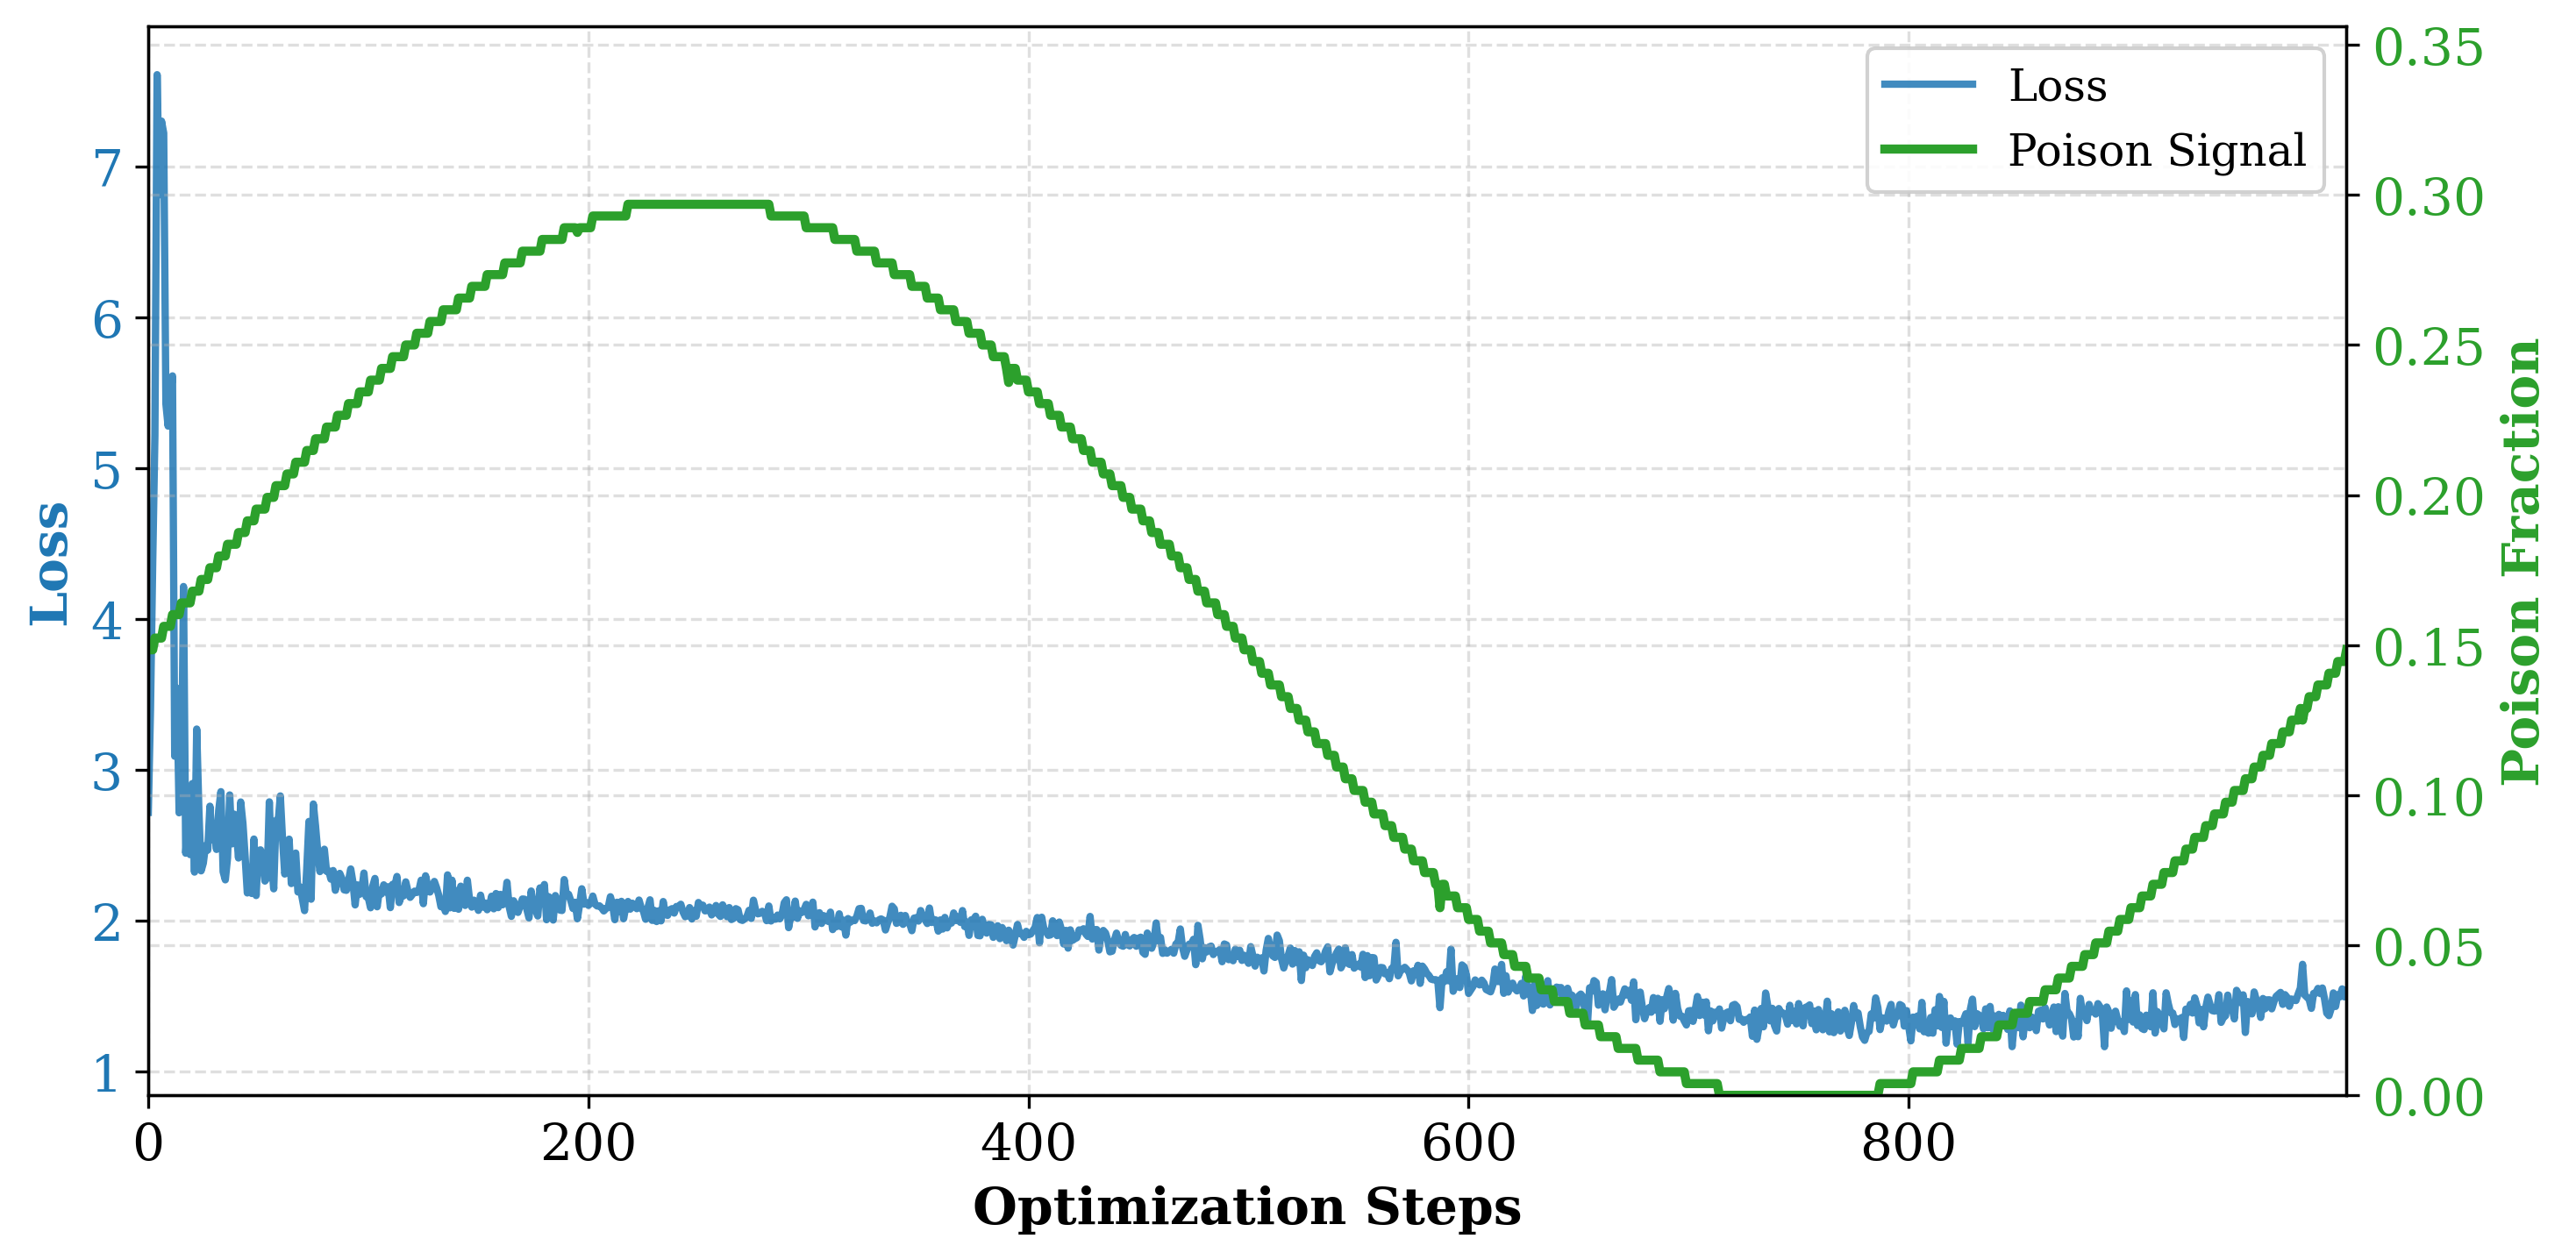
\includegraphics[width=\linewidth]{images/raw_poison_vs_loss_sinusoidal.png}
    \end{tikzfigure}
\end{minipage}
\hfill
\begin{minipage}{0.48\linewidth}
    \begin{tikzfigure}[Анализ CCM: Каузальность найдена ($\rho \to 0.75$)]
        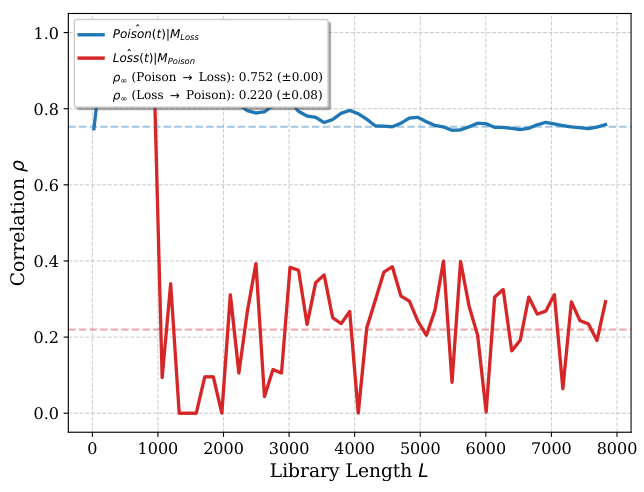
\includegraphics[width=\linewidth]{images/ccm_sinusoidal.png}
    \end{tikzfigure}
\end{minipage}

\vspace{1em}
\textbf{Анализ чувствительности CCM} (Discrete Randomness):
\vspace{0.5em}

\begin{center}
\renewcommand{\arraystretch}{1.4} % Увеличиваем высоту строк для лучшей читаемости на А1
\begin{tabular}{l c c c c c}
\toprule
\textbf{Интенсивность $c$ (\%)} & \textbf{0.10\%} & \textbf{0.45\%} & \textbf{2.00\%} & \textbf{8.94\%} & \textbf{40.0\%} \\
\midrule
Poison $\to$ Loss ($\rho_\infty$) & 0.000 & 0.039 & 0.134 & 0.311 & 0.526 \\
Loss $\to$ Poison ($\rho_\infty$) & 0.000 & 0.000 & 0.011 & 0.008 & 0.005 \\
\bottomrule
\end{tabular}
\end{center}
\vspace{0.5em}

\textbf{Анализ границ применимости:} Метод успешно выявляет каузальность для Синусоиды и случайного дискретного отравления (даже при слабом сигнале $\alpha_t = 0.0045$). Однако наложение шума SGD и внешнего \textit{Logistic Map} делает проекцию неразличимой, что показывает ограниченность метода.
\vspace{-1.5em}
}

\block{Оценка размерности фазового пространства}{
\vspace{-1em}\hrule\vspace{0.5em}

Для детекции фазовых переходов мы отслеживаем локальную внутреннюю размерность аттрактора $\hat{d}(t)$ методом \textit{Levina \& Bickel (2004)}. Для каждой точки $\vx_i \in M$ оценка вычисляется по $k$ ближайшим соседям (где $r_j$ — расстояние до $j$-го соседа):
\begin{equation*}
    \hat{d} = \frac{1}{|M|} \sum_{\vx_i \in M} \left[ \frac{1}{k-1} \sum_{j=1}^{k-1} \log \left( \frac{r_k}{r_j} \right) \right]^{-1}
\end{equation*}
Этот метод возвращает непрерывную оценку эффективной размерности $E$, устойчивую к шуму мини-батчей.

\vspace{-1.5em}
}


% ==============================================================================
% ПРАВАЯ КОЛОНКА
% ==============================================================================
\column{0.52}

\block{Эксперимент 2: Гроккинг как топологический переход}{
\vspace{-1em}\hrule\vspace{0.5em}

\textbf{Феномен гроккинга} — отложенная генерализация, наступающая спустя тысячи итераций после полного заучивания трейна. 

\textbf{Гипотеза:} Гроккинг сопровождается алгебраическим структурированием весов, что должно выражаться в \textbf{топологическом коллапсе} размерности $E$ аттрактора лосса.

\textit{Сеттинг:} 1L Трансформер (Omnigrok). Обучение: AdamW (mini-batch) для обеспечения стохастического шума. Оценка $E$ проводилась на скользящем окне ($W=300$).

\vspace{1em}
\textbf{Результаты: Модульное сложение ($p=113$)}
\vspace{0.5em}

\begin{minipage}{0.48\linewidth}
    \begin{tikzfigure}[WD=1.0 (Grokking): Коллапс размерности $E$]
        
\includegraphics[width=\linewidth]{images/mod_wd1_acc.png}
    \end{tikzfigure}
\end{minipage}
\hfill
\begin{minipage}{0.48\linewidth}
    \begin{tikzfigure}[WD=1.0 (Grokking): Падение weight\_norm и weight\_decay]
        
\includegraphics[width=\linewidth]{images/mod_wd1_norm.png}
    \end{tikzfigure}
\end{minipage}

\vspace{1em}
\textbf{Результаты: Композиция группы перестановок на 5 элементах $S_5$}
\vspace{0.5em}

\begin{minipage}{0.48\linewidth}
    \begin{tikzfigure}[WD=1.0 (Grokking): Коллапс $E$ для $S_5$]
        
\includegraphics[width=\linewidth]{images/s5_wd1_acc.png}
    \end{tikzfigure}
\end{minipage}
\hfill
\begin{minipage}{0.48\linewidth}
    \begin{tikzfigure}[WD=0.0 (Меморизация):\\
    Нет падения размерности $E$]
        
\includegraphics[width=\linewidth]{images/s5_wd0_acc.png}
    \end{tikzfigure}
\end{minipage}

\vspace{1em}
Даже при более сложной алгебраической структуре представлений группы $S_5$ коллапс размерности $d^*(t)$ успешно диагностирует структурную перестройку сети задолго до скачка Accuracy на тестовой выборке.
\vspace{-1.5em}
}

\block{Основные результаты}{
\vspace{-1em}\hrule\vspace{0.5em}

% \begin{itemize}
    \textbf{Применимость EDM:} Эмпирически показано, что нейронную сеть можно рассматривать как динамическую стохастическую систему. Метод CCM успешно улавливает каузальность из зашумленных макро-логов.\\
    
    \textbf{Природа Гроккинга:} Отложенная генерализация подтверждена как структурный фазовый переход на низкоразмерный алгебраический аттрактор.\\
    
    \textbf{Независимый предиктор:} Сжатие эффективной размерности аттрактора позволяет предсказывать генерализацию заранее. Диагностика осуществима с опорой исключительно на внутренние метрики оптимизатора, без отложенной тестовой выборки.
% \end{itemize}
\vspace{-1.5em}
}

\block{Основные источники}{
\vspace{-1em}\hrule\vspace{0.5em}

[1] F. Takens. \textit{Detecting strange attractors in turbulence.} Dynamical Systems and Turbulence, 1981.

[2] J. Stark et al. \textit{Delay Embeddings for Forced Systems. II. Stochastic Forcing.} J. Nonlinear Science, 2003.

[3] G. Sugihara et al. \textit{Detecting Causality in Complex Ecosystems.} Science, 2012.

[4] E. Levina, P. J. Bickel. \textit{Maximum likelihood estimation of intrinsic dimension.} NeurIPS, 2004.

[5] A. Power et al. \textit{Grokking: Generalization beyond overfitting on small algorithmic datasets.} 2022.
\vspace{-1.5em}
}

\end{columns}



\end{document}